\documentclass[10pt,twocolumn]{witseiepaper}

\usepackage{KJN}
\hyphenation{op-tical net-works semi-conduc-tor}
\usepackage{graphicx}
\usepackage[export]{adjustbox}
\usepackage{fancyhdr}
\usepackage{url}
\usepackage{amsmath}
\usepackage{listings}
\usepackage{algorithm}
\usepackage{algorithmic}
\usepackage{lipsum}
\usepackage{bookmark}

%----------------------------------------------------------------------------------------
%	PDF INFORMATION
%----------------------------------------------------------------------------------------
\ifpdf
\pdfinfo{
/Title (Project Plan: Image Compression based on Non-Parametric Sampling in Noisy Environments)
/Author (Group 19G01)
/CreationDate (01/07/2019)
/Subject (ELEN4012)
/Keywords (ELEN4012, Laboratory Project, Image Compression, 4th Year)
}
\fi

%%%%%%%%%%%%%%%%%%%%%%%%%%%%%%%%%%%%%%%%%%%%%%%%%%%%%%%%%%%%%%%%%%%%%%%%%%%%%%%
\begin{document}

%----------------------------------------------------------------------------------------
%	TITLE
%----------------------------------------------------------------------------------------

\title{PROJECT PLAN\\ Image Compression based on Non-Parametric Sampling in Noisy Environments}

\author{Group 19G01: Kishan Narotam (717 931) \& Nitesh Nana (720 064)
\thanks{School of Electrical \& Information Engineering, University of the
Witwatersrand, Private Bag 3, 2050, Johannesburg, South Africa}
}


%----------------------------------------------------------------------------------------
%	ABSTRACT
%----------------------------------------------------------------------------------------
\abstract{}

\keywords{DCT, Decoding, Encoding, Holes, Image Compression}


\maketitle
\thispagestyle{empty}\pagestyle{empty}


%----------------------------------------------------------------------------------------
%	MAIN BODY OF REPORT
%----------------------------------------------------------------------------------------
\section{INTRODUCTION}
\label{sec: Introduction}
A project plan is a formal document that forms a guideline of the project that will ensure the overall success and completion of the project~\cite{Techopedia}. Planning the project involves looking at three fundamental aspects of the project:
\begin{itemize}
\item Scope: what are the objectives of the project and how it will be completed
\item Cost: how much money is allocated, budgeted and spent over the course of the project
\item Time: the time taken to execute the project to a point of completion~\cite{PM}.
\end{itemize}

In the report that follows, a project plan is created for the telecommunications project of \emph{image compression based on non-parametric sampling in noisy environments}. Firstly, the project specifications are defined, followed by a brief look into existing models. Subsequently, the proposed strategy for the project is done with a cost and time management which is discussed in order for the project to be completed on time within a specified budget.

%%%%%%%%%%%%%%%%%%%%%%%%%%%%%%%%%%%%%%%%%%%%%%%%%%%%%%%%%%%%%%%%%%%%%%%%%%%%%%%
%
\section{PROJECT SPECIFICATIONS}
\label{sec: Project Specs}
The aim of the project is to create a robust scheme for determining multiple holes that may be received in an image and appropriately fill these holes. in addition, the image may be subject to random burst errors which need to be identified and corrected.

An image will be chosen for compression utilizing a compression technique and creating holes in the image and after transmitting, filling of those holes will result in the original image. The holes will be created manually making use of current compression algorithms (such as fractal compression for example). Once the holes are created, the image will be transmitted via a simple channel that will introduce errors randomly. The image will be received at the receiver, and knowing where the holes are present, will fill them accordingly using a different algorithm. The receiver will also have to deal with random errors that may have occurred from the channel. The received image with the filled holes will be reconstructed and presented as the final image which should coincide with the original image.

%%%%%%%%%%%%%%%%%%%%%%%%%%%%%%%%%%%%%%%%%%%%%%%%%%%%%%%%%%%%%%%%%%%%%%%%%%%%%%%
%
\section{EXISTING MODELS}
\label{sec: Existing Models}
Image compression is an application of data compression where an image file is encoded with a few bits with the overall goal of reducing the size of the image file compared to that of the original~\cite{ImageComp}. There are two main techniques of image compression:
\begin{itemize}
\item Lossless
\item Lossy
\end{itemize}

\subsection{Lossless}
\label{sec: Lossless}
Lossless compression allows the original form of data to be reproduced, thus meaning that the original data from the file before compression is preserved~\cite{Loss}. Some of the current lossless compression techniques include:
\begin{itemize}
\item Run-Length encoding
\item Huffman encoding
\item Shannon-Fano encoding
\item Arithmetic
\item Dictionary based.
\end{itemize}


\subsection{Lossy}
\label{sec: Lossy}
Lossy compression removes some of the data from the original file, resulting in an overall reduction of the size of the file~\cite{Loss}. The non-useful parts of the data that is not noticeable is removed, thus reducing the overall quality of the data and file. Some of the current lossy compression techniques include:
\begin{itemize}
\item Lossy predictive
\item Vector Quantization
\item Transform Coding
\item Block transform
\item DCT/DWT
\item JPEG.
\end{itemize}

%%%%%%%%%%%%%%%%%%%%%%%%%%%%%%%%%%%%%%%%%%%%%%%%%%%%%%%%%%%%%%%%%%%%%%%%%%%%%%%
%
\section{PROPOSED STRATEGY}
\label{sec: Proposed Strategy}
The proposed solution will be implemented in MATLAB and can be broken down into two sides:
\begin{itemize}
\item Encoder side
\item Decoder side.
\end{itemize}
In conjunction with this, a simple channel will be created and random errors will be introduced after the image is encoded. Figure~\ref{fig: Block Diagram} shows the basic framework and block diagram of the proposed solution that will be implemented.

\begin{figure}[h!]
\renewcommand{\thefigure}{\arabic{figure}}
\hspace{-0.5cm}
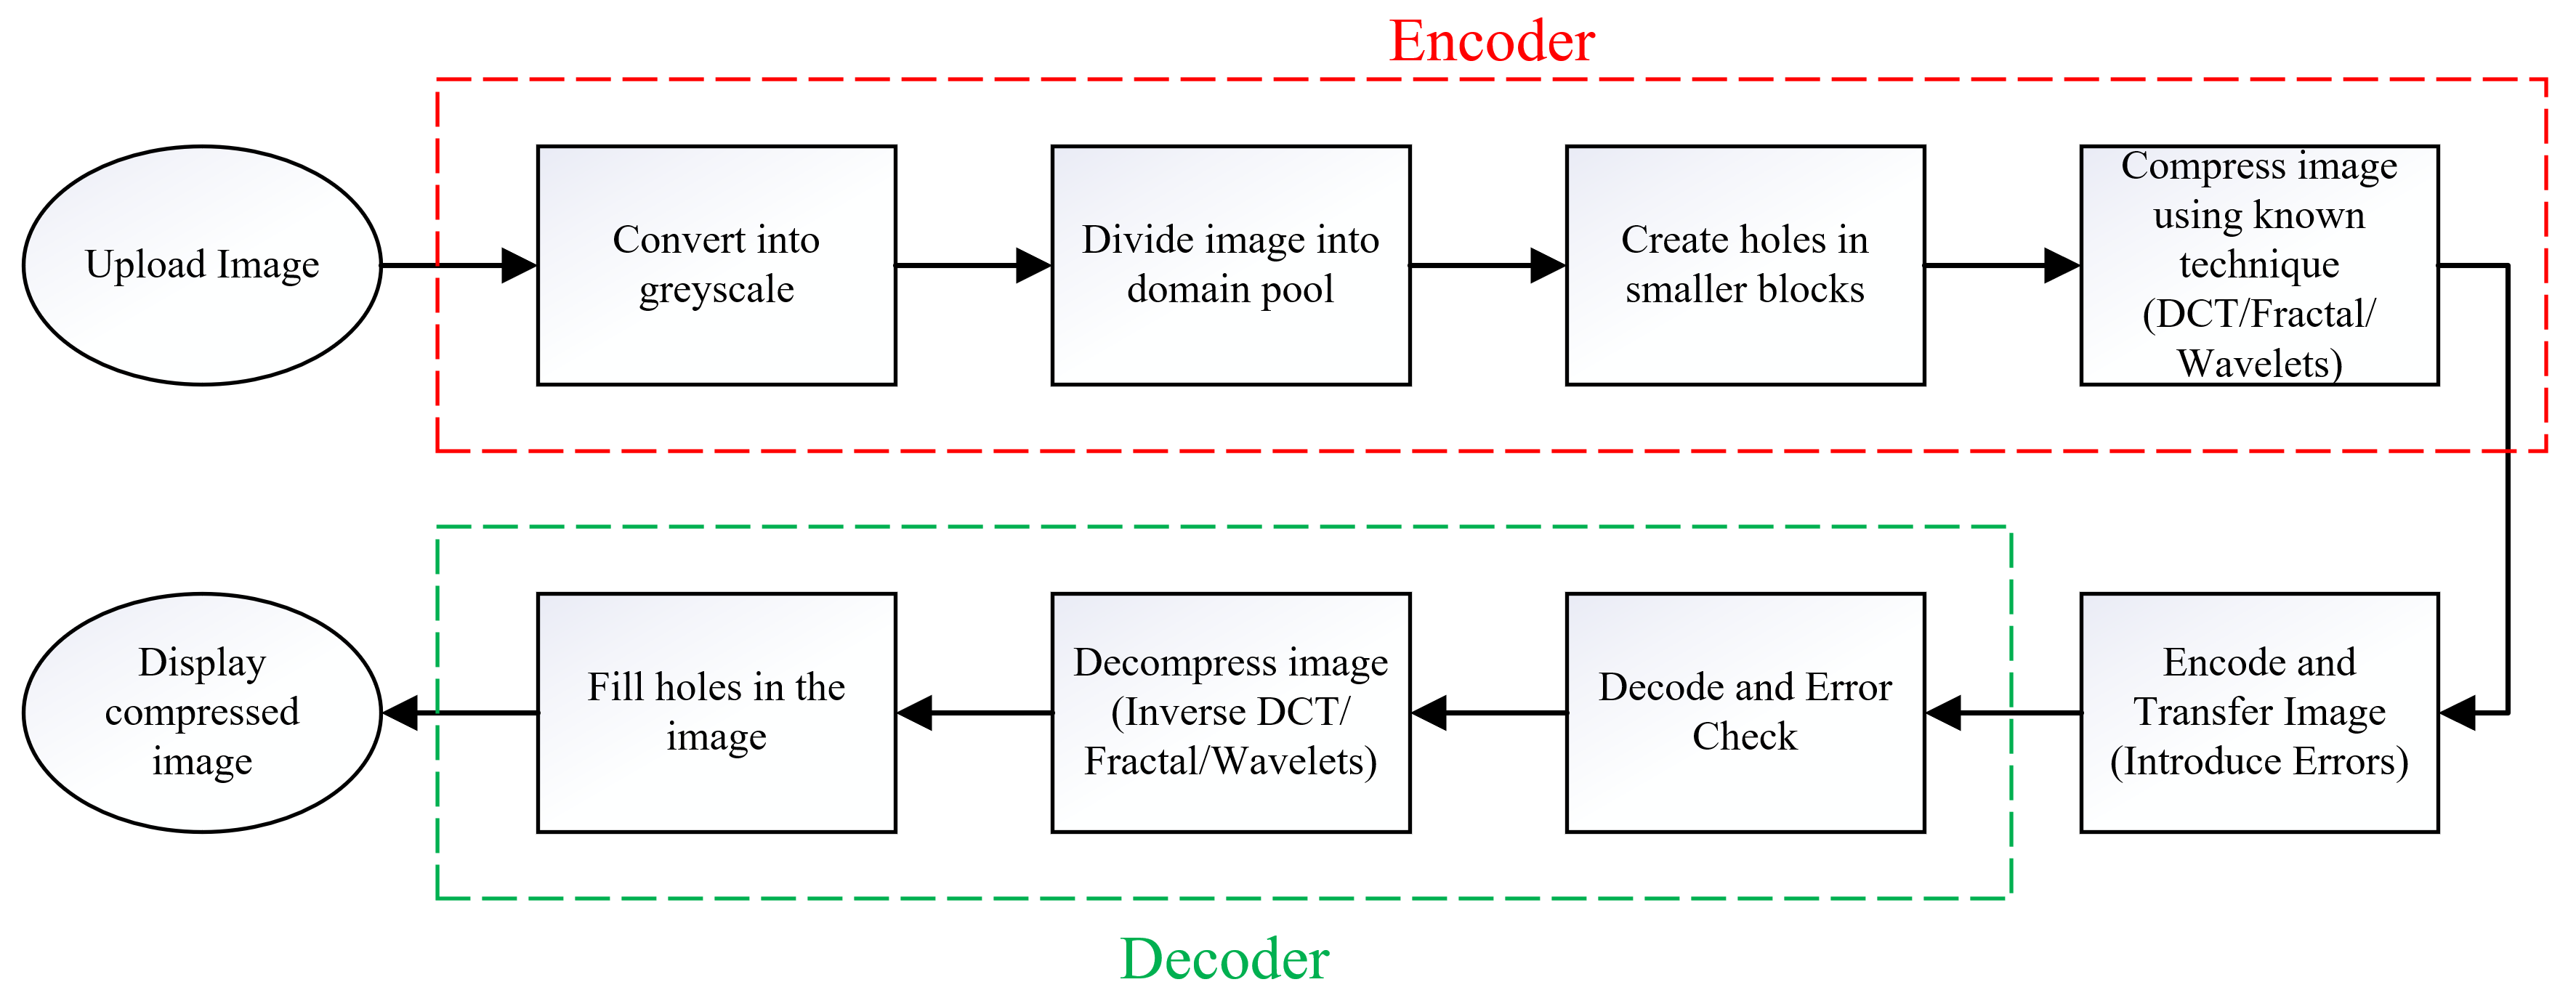
\includegraphics[scale=0.16]{BlockDiagram.png}
\caption{Block diagram of the proposed strategy}
\label{fig: Block Diagram}
\end{figure}

\subsection{Step 1: Loading/Reading an Image into MATLAB}
\label{sec: Step 1}
Firstly, an image is loaded into MATLAB, and a PNG or BMP image is specifically chosen with the dimensions $M\times N$, where $M$ and $N$ are divisible by 8. A PNG or BMP image is used as a JPEG image, is already a compressed image via the DCT image compression technique. Figure~\ref{fig: Step 1} shows an example of the image that can be used. 
\begin{figure}[h!]
\renewcommand{\thefigure}{\arabic{figure}}
\centering

\includegraphics[scale=0.3, frame]{Step1.png}
\caption{$128\times 128$ image that will be loaded}
\label{fig: Step 1}
\end{figure}

\subsection{Step 2: Convert the image to greyscale}
\label{sec: Step 2}
The loaded image is converted to greyscale, and the reason for this is because an image that has been imported into MATLAB creates a 3-dimensional array where the first two elements of the array represent the dimensions of the image and the third dimension is the colour map. Converting the image to a greyscale one, creates a 2-dimensional array, which are simply the dimensions of the image, where each array value correlates to the specific integer value of that specific pixel. Figure~\ref{fig: Step 2} shows an example of the outcome of converting the image to greyscale.
\begin{figure}[h!]
\renewcommand{\thefigure}{\arabic{figure}}
\centering

\includegraphics[scale=0.3, frame]{Step2.png}
\caption{Image after it has been greyscaled in MATLAB}
\label{fig: Step 2}
\end{figure}

\subsection{Step 3: Divide the image into the domain pool}
\label{sec: Step 3}
The image is now divided into smaller $8\times 8$ blocks, creating the domain pool. Once the image has been divided into smaller blocks, we index each block from the top left starting from 1 and increment each index by one, moving left-to-right, top-to-bottom. The reason for creating such an index is so that the receiver will be able to determine which smaller block in the domain pool contains holes so that the receiver can fill these holes. Figure~\ref{fig: Step 3} shows an example of the loaded image having a domain pool of $256$ blocks.
\begin{figure}[h!]
\renewcommand{\thefigure}{\arabic{figure}}
\centering

\includegraphics[scale=0.4, frame]{Step3.jpg}
\caption{Smaller $8\times 8$ blocks creating the domain pool}
\label{fig: Step 3}
\end{figure}

\subsection{Step 4: Create holes in the smaller blocks}
\label{sec: Step 4}
With the domain pool created, holes are created by starting at the center square within the $8\times 8$ block. Starting off with the center $2\times 2$ square, the average value of those 4 pixels are calculated. If the average value is within $\pm 5\ or\ 10$ of each pixel value, a hole can be created in those 4 pixels. A larger square in the same $8\times 8$ block is checked with a size of $4\times 4$. The average of these pixels are calculated and as before compared to each value of the center square. This can continue until we reach a center square size of $6\times 6$, which we will define as the largest hole that can be made. Figure
\begin{figure}[h!]
\renewcommand{\thefigure}{\arabic{figure}}
\centering
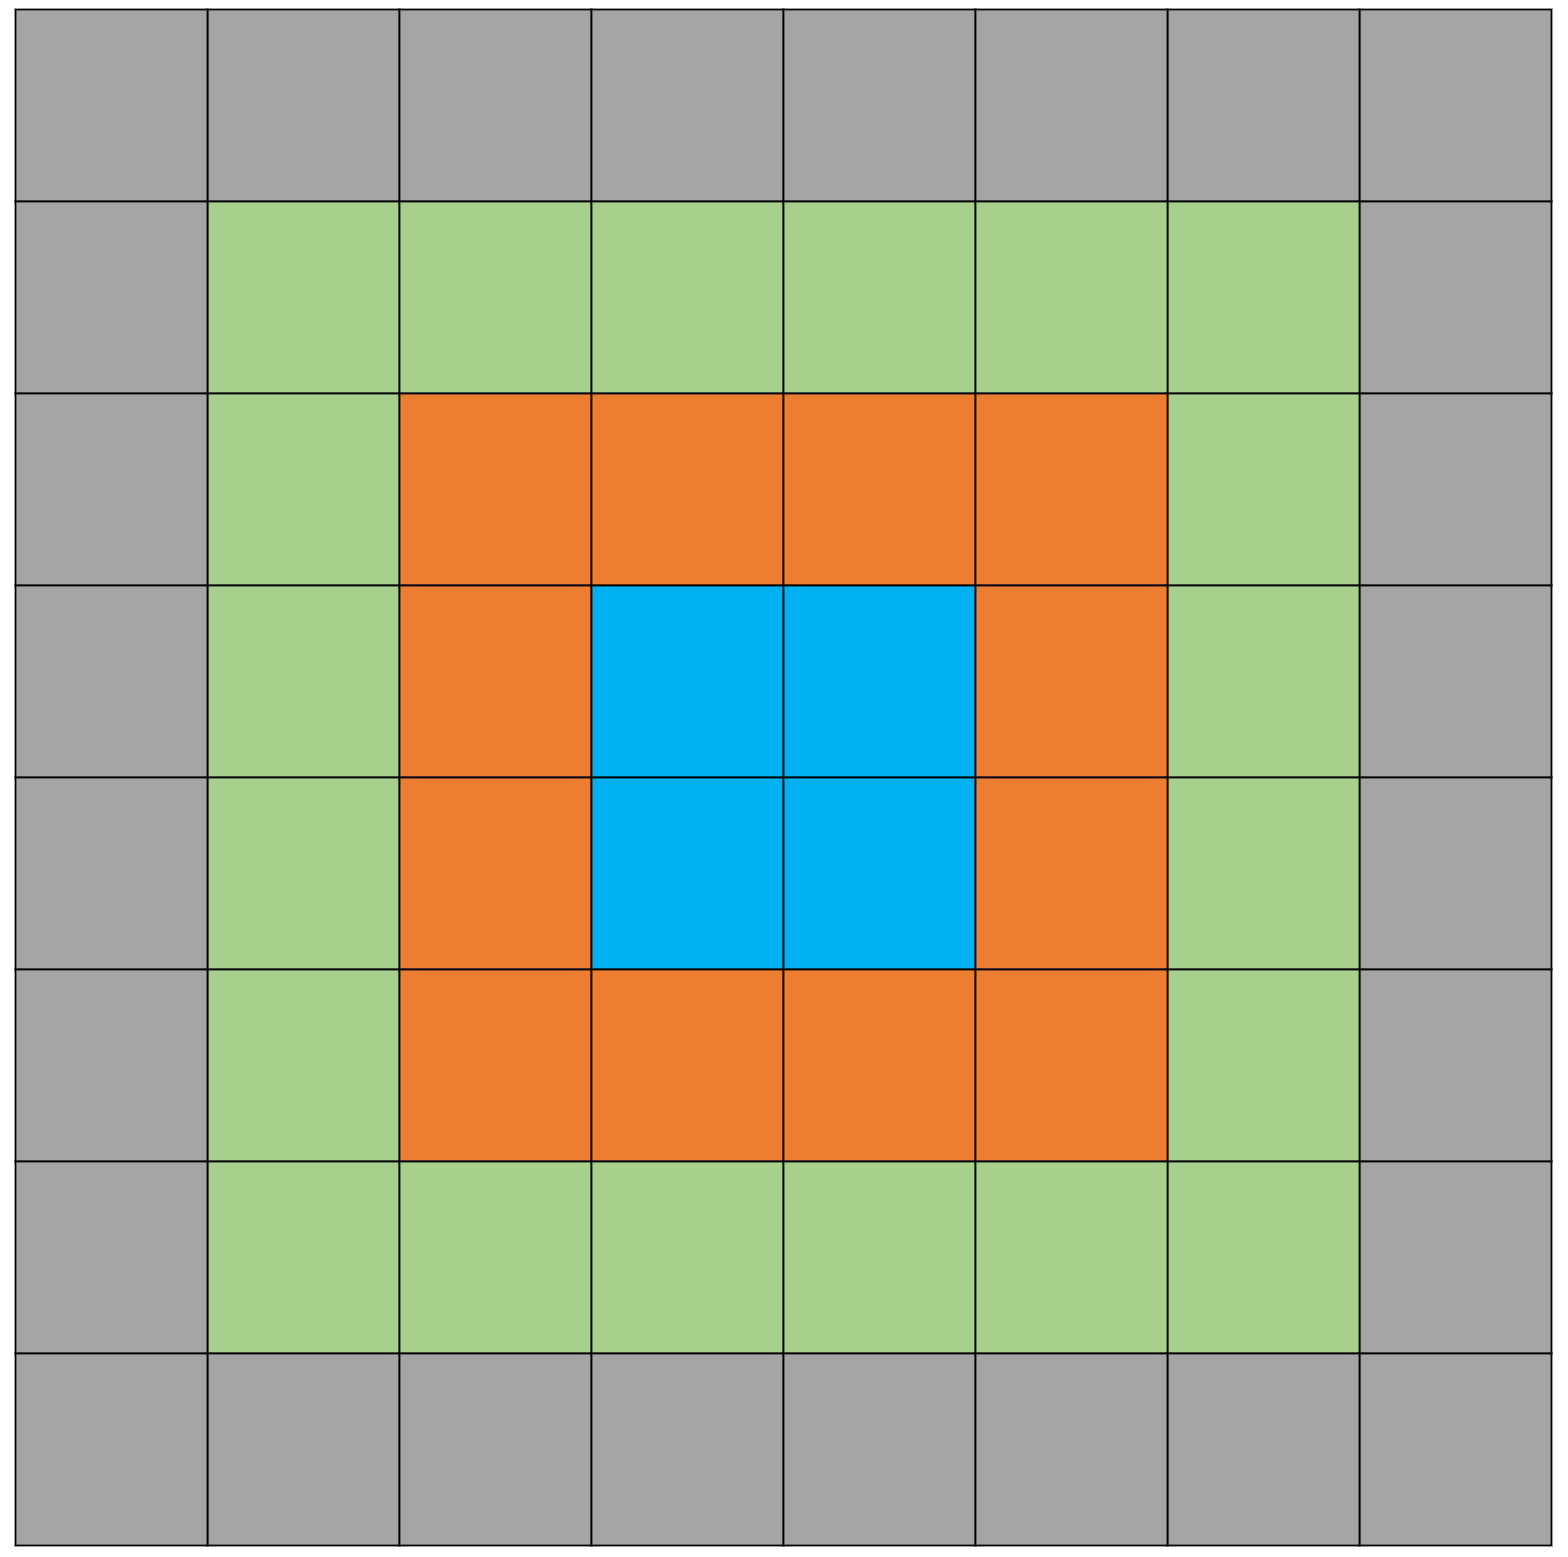
\includegraphics[scale=1.5]{Grid.png}
\caption{How a $8\times 8$ block (black square) will be checked for hole creation starting with the purple square.}
\label{fig: Grid}
\end{figure}

\subsection{Index block if the hole has been created}
\label{sec: Index Block}
If a hole has been created in a specific block in the domain pool, a one-dimensional array will be created with the value of the block index. This array will be transmitted with the image itself, so that when received by the receiver, it will have a list of the blocks in the domain pool that contain a hole.

\subsection{Step 5: Compress image using a known technique (DCT)}
\label{sec: Step 5}
The DCT compression technique will be utilized for the compression of the image. DCT will be performed on each block in the domain pool, and DCT is done on $8\times 8$ matrix, which is the reason the domain pool is made up of multiple $8\times 8$ blocks and that an image where the dimensions are divisible by 8 is chosen. The image is now compressed and can be transmitted into the channel.

\subsection{Step 6: Encode and Transfer image}
\label{sec: Step 6}
The image is encoded as a binary message, and when transmitted through the channel, errors are randomly introduced. The data that will be sent through the channel will be a bit stream and the errors introduced will be based off of a byte with a probability of $10^{-3}$ where the byte can then be randomized. Alternatively, each bit can be random selected to be prone to an error and the bit value flipped. 

\subsection{Step 7: Decode and Error Check}
\label{sec: Step 7}
Identification of the location of the errors is required. First, identifying the errors are required, and if detected must be corrected and then the image can be decoded. The image will be converted from a bit stream into its 2-dimensional matrix.

\subsection{Step 8: Decompress (Inverse DCT)}
\label{sec: Step 8}
Since DCT compression was used, we now perform the inverse DCT to obtain the compressed image and its respective values in the 2-dimensional matrix.

\subsection{Step 9: Fill holes in the image}
\label{sec: Step 9}
With the one-dimensional array sent across the channel, the blocks within the domain pool that contain the holes can be identified. Starting at outer pixels, the average pixel value of the square is calculated, and that will fill the inner pixels where the hole was created.

%%%%%%%%%%%%%%%%%%%%%%%%%%%%%%%%%%%%%%%%%%%%%%%%%%%%%%%%%%%%%%%%%%%%%%%%%%%%%%%
%
\section{COST MANAGEMENT}
\label{sec: Cost Management}
The nature of this project is software based, and thus the total costs are minimal to none. Licences for the MATLAB software is already provided as a student licence by the university, and personal computers or laptops will be used.

%%%%%%%%%%%%%%%%%%%%%%%%%%%%%%%%%%%%%%%%%%%%%%%%%%%%%%%%%%%%%%%%%%%%%%%%%%%%%%%
%
\section{TIME MANAGEMENT}
\label{sec: Time Management}
The Project window runs from 15 July 2019 until 29 August 2019. The proposed timeline of events and duration of these events can be seen in Figure~\ref{fig: Gantt}. Based on the planned approximated time that is allocated to each task, this indicates that keeping to a tight schedule is required.


%%%%%%%%%%%%%%%%%%%%%%%%%%%%%%%%%%%%%%%%%%%%%%%%%%%%%%%%%%%%%%%%%%%%%%%%%%%%%%%
%
\section{CONCLUSION}
\label{sec: Conclusion}


%%%%%%%%%%%%%%%%%%%%%%%%%%%%%%%%%%%%%%%%%%%%%%%%%%%%%%%%%%%%%%%%%%%%%%%%%%%%%%%
%
\begin{thebibliography}{}

%**************************Section**************************%

\bibitem{Techopedia}
Techopedia; \emph{What is a Project Plan? - Definition from Techopedia}; \url{https://www.techopedia.com/definition/24775/project-plan}; Last Accessed: 02/07/2019

\bibitem{PM}
Heerkins, G R; \emph{Project Management}; McGraw-Hill; New York, NY, United States; 1st Edition, 2001

\bibitem{ImageComp}
Wei-Yi Wei; \emph{An Introduction to Image Compression}; Graduate Institute of Communication Engineering; National Taiwan University; Taipei, Taiwan, ROC

\bibitem{Loss}
Chapman, C; \emph{Everything You Need to Know About Image Compression | The JotForm Blog}; \url{https://www.jotform.com/blog/everything-you-need-to-know-about-image-compression/}; Last Accessed: 02/07/2019

\end{thebibliography}

\onecolumn
\begin{figure}[h!]
\renewcommand{\thefigure}{\arabic{figure}}
\centering
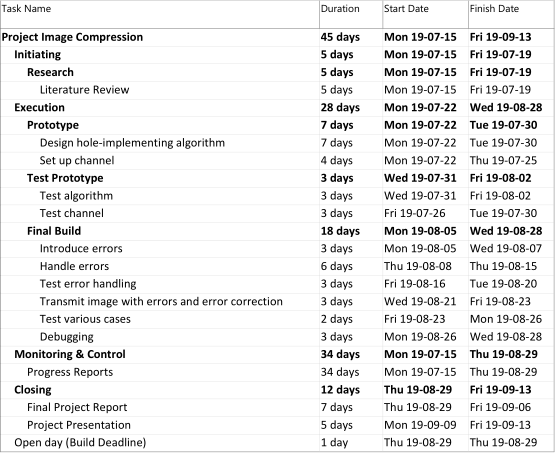
\includegraphics[scale=1]{Gantt.png}
\caption{Table showing the tasks and time allocated in completing the project}
\label{fig: Task Time Management}
\end{figure}

\begin{figure}[h!]
\renewcommand{\thefigure}{\arabic{figure}}
\centering
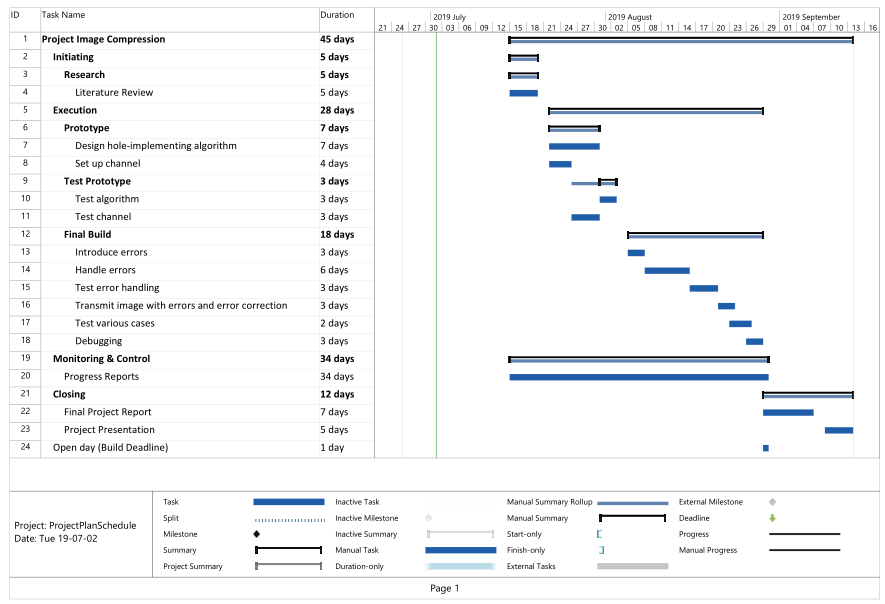
\includegraphics[scale=0.8]{gantt1.png}
\caption{Gantt chart showing the tasks and time allocated in completing the project}
\label{fig: Gantt}
\end{figure}

\end{document}

" vim: ts=4
" vim: tw=78
" vim: autoindent
" vim: shiftwidth=4
